\documentclass[a4paper,10pt]{article}
\usepackage[utf8]{inputenc}
\usepackage{subcaption}
\usepackage{xcolor}
\usepackage{float}
\usepackage{graphicx}
\usepackage{listings}   %for code
\usepackage[font={small,bf}]{caption}
\usepackage{authblk}    %for affil in title page
\usepackage[colorlinks=true,linkcolor=blue,citecolor=red, urlcolor=red]{hyperref}
\usepackage{color}
\usepackage[english]{babel}
\usepackage{amsmath}

\definecolor{codegreen}{rgb}{0,0.6,0}
\definecolor{codegray}{rgb}{0.5,0.5,0.5}
\definecolor{codepurple}{rgb}{0.58,0,0.82}
\definecolor{backcolour}{rgb}{0.97,0.97,0.97}

\lstdefinestyle{mystyle}{
    backgroundcolor=\color{backcolour},
    commentstyle=\color{codegreen},
    keywordstyle=\color{blue},
    numberstyle=\tiny\color{codegray},
    stringstyle=\color{codepurple},
    basicstyle=\ttfamily\footnotesize,
    breakatwhitespace=false,
    breaklines=true,
    captionpos=b,
    keepspaces=true,
    numbers=left,
    numbersep=5pt,
    showspaces=false,
    showstringspaces=false,
    showtabs=false,
    tabsize=2,
    morecomment=[l][\color{codegreen}]{\#}
}

\lstset{style=mystyle}

\begin{document}

\begin{titlepage} % Suppresses displaying the page number on the title page and the subsequent page counts as page 1
	
	\raggedleft % Right align the title page
	
	\rule{1pt}{\textheight} % Vertical line
	\hspace{0.02\textwidth} % Whitespace between the vertical line and title page text
	\parbox[b]{0.75\textwidth}{ % Paragraph box for holding the title page text, adjust the width to move the title page left or right on the page
		
		{\Huge\bfseries TDT4287}\\[2\baselineskip] % Title
		{\large\textit{Preprocessor for high throughput sequencing reads}}\\[4\baselineskip] % Subtitle or further description
		{\Large\textsc{roc salvador\\marc falcón}} % Author names, lower case for consistent small caps
		
		\vspace{0.5\textheight} % Whitespace between the title block and the publisher
		
		{\noindent \today}\\[\baselineskip] % Date
	}

\end{titlepage}


\tableofcontents

\newpage

\section{Task 1} \label{task1}

\paragraph{} The first task consists of developing an algorithm that identifies all the sequences in S that contain suffixes that perfectly match a prefix of the given adapter sequence.

\subsection{Trie}

\paragraph{} For Task 1 [\ref{task1}] and Task 2 [\ref{task2}] we used a trie as a data structure to store the prefixes of the adapter sequence.
A trie is structured as a tree, where each node contains a letter and each node has children that represent the successive letters of the words stored in the trie. 
You can see an example in the following picture [\ref{trie-example}].
\begin{figure}[H]
    \centering
    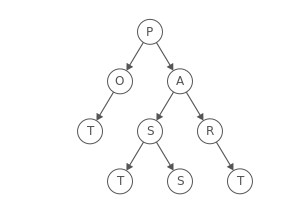
\includegraphics[width=7cm, height=5cm]{images/trie.png}
    \caption{Trie for "part", "pot", "past" and "pass"}
    \label{trie-example}
\end{figure}

\begin{lstlisting}[language=c++, caption=Our trie implementation]
class Trie {
    struct Node {
        // Childs of the current node,
        // in our case can only be 4: 'A', 'C, 'G' and 'T'
        // A child is NULL if it does not exist
        Node*[] childs = Node*[4];
        // True if a node is a valid end of a word, false otherwise
        bool isWordEnd;         
        // True if a node is a leaf of the tree, false otherwise
        bool isLeaf;            
    };

    Node* root;
};
\end{lstlisting}

\paragraph{} The trie construction is done in linear time with respect to the size of the text that represents. In our case the construction of the trie of the suffix of the reversed adapter sequence (see example [\ref{s-example-trie}]) is $O(\dfrac{k\cdot(k-1)} {2})$ that is equal to the length of all suffixes, where $k = |adapter_sequence|$.

\subsection{Perfect suffix-prefix match} \label{perfect-spm}

To solve the prefix-suffix problem, we use the algorithm presented next, we have to create a trie with all the suffixes of the reversed adapter sequence and then the sequences have to be reversed when searched.

Example: \label{s-example-trie}
$$ A = ACGACG $$
$$ reversedA = GCAGCA $$
$$ S = TACG $$
$$ reversedS = GCAT $$

Trie of suffixes of $reversedA$:
$$root-G-C-A(word end)-G-C-A(wordend)$$
$$root-C-A(wordend)-G-C-A(wordend)$$
$$root-A(wordend)-G-C-A(wordend)$$

If we search in the trie the $reversedS$ we will get a match since the search will reach a $word end$.
$$\mathbf{root-G-C-A(word end)}-G-C-A(wordend)$$

\paragraph{} The algorithm that we have used is quite simple.
It starts from the root and checks if there is any child with the first letter of the input string $s$, if that child exists it moves to the child and checks if there is any child with the second letter of the $s$...
If the actual node corresponds to an end of a word in the trie, the actual length becomes the longest match.
This is done until it reaches the end of $s$, or there is no child with the next letter of $s$, or the node is a leaf of the trie.

\begin{lstlisting}[language=c++, caption=Iterative algorithm for perfect suffix-prefix match]
// This function returns the length of the longest match between the string s and the text stored in the trie 
int longestPerfectMatch(string s) {
    int longestMatch = 0, remainder = 0;
    // Get the root of the trie
    Node* node = root;
    string nextStr = s;
    // This function returns [0..4] for ['A','C','G','T']
    int index = nuclToInt(nextStr[0]);

    // Iterate while we find a path
    while (node->childs[index] != NULL) {
        node = node->childs[index];
        ++remainder;
        nextStr = nextStr[1:];
        index = nuclToInt(nextStr[0]);
        // If we reach a word end acomulate all the remainder that 
        // we counted
        if (node->isWordEnd) {
            longestMatch += remainder;
            remainder = 0;
        }

        if (node->isLeaf or nextStr == "") return longestMatch;
    }
    return longestMatch;
}
\end{lstlisting}

\paragraph{} The running time of this algorithm is linear with respect to the size of the input string $s$, $O(m)$, where $m = |s|$, since we iterate until $s$ is traversed or the actual node has no more matches. The practical running time we have is 1.618s for the 1000000 sequences in s\_3\_sequence\_1M.txt.

\subsection{Results}

\begin{table}[H]
    \centering
    \begin{tabular}{| c | c |}
        \hline
        Matches & 100\% match \\
        \hline
        \hline
        646368 & 132149 \\
        \hline
    \end{tabular}
    \caption{Matches obtained}
\end{table}

\begin{figure}[H]
    \centering
    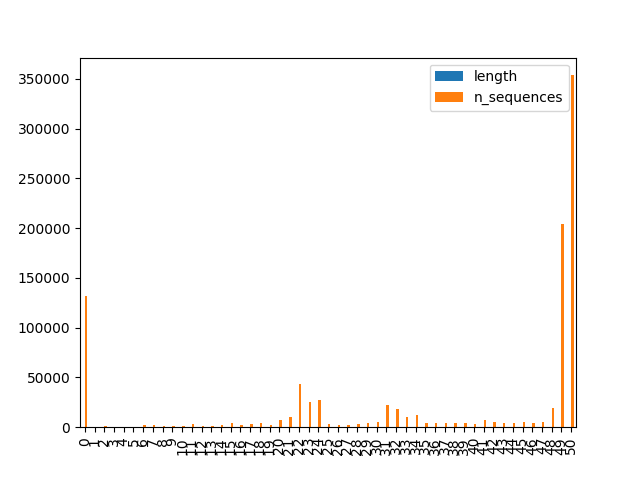
\includegraphics[width=12cm]{images/length-distr.png}
    \caption{Length distribution of the sequences after removing the adapter fragments}
    \label{length-distr}
\end{figure}

\newpage

\section{Task 2} \label{task2}

\paragraph{} The second task consists of developing an algorithm that identifies all the sequences in S that contain suffixes that match a prefix of a and where this suffix can contain up to a given percentage of mismatches to the prefix of the given adapter sequence.

\subsection{Imperfect suffix-prefix match} \label{imperfect}

\paragraph{} For the second task we based our algorithm on a recursive DFS. It traverses the trie, and it increases the error count when there is a mismatch.
Since we want the full-length match, the actual node checks the maximum match length of the children.
The length is increased when a new node is visited but the maximum length is only updated when a node corresponds to a word ending.
The trie and the $s$ are the same as in the previous task [\ref{perfect-spm}].
The call to get the length of a match of a sequence's suffixes and the adapter sequence's prefixes would be \texttt{longestImperfectMatch(reversedSequence, 0, 0, 0, trieRoot)}.

\begin{lstlisting}[language=c++, caption=Recursive algorithm for imperfect suffix-prefix match, label=im]
int longestImperfectMatch(string s,
                          int longest,
                          int length,
                          int errors,
                          Node* node) {
    // Quit the search if the errors are greater than the
    // maximum errors the total sequence can have
    if (errors > maxTotalErrors) return longest;

    int maxErrors = length * (percentage / 100.0);

    // If the sequence is traversed, end the search and
    // update the maximum match length if necessary
    if (s == "") {
        if (node->isWordEnd and errors <= maxErrors) 
            longest = max(length, longest);
        return longest;
    }

    int index = nuclToInt(s[0]);
    string nextStr = s[1:];

    // If the actual node is an end of a word update the 
    // longest match
    if (node->isWordEnd and errors <= maxErrors) 
        longest = max(length, longest);

    ++length;

    // Search for the longest match among the children
    for (int i = 0; i < node->childs.size(); ++i) {
        Node* child = node->childs[i];
        if (child != NULL) {
            // If the letters match do not increase the error
            if (i == index) 
                longest = max(longest, longestImperfectMatch(nextStr,longest, length, errors, child));
            // Else increase the error counter
            else 
                longest = max(longest, longestImperfectMatch(nextStr, longest, length, errors+1, child));
        }
    }
    return longest;
}
\end{lstlisting}

\paragraph{} \label{rn-im} The worst asymptotic running time of this algorithm is $O(\dfrac{k\cdot(k-1)} {2})$, where $k = |adapter\_sequence|$, since it is the maximum size that the trie could have when we add all the suffixes.
The practical running time that we got depends on the percentage of errors since the algorithm quits the search when the number of errors is bigger than the total maximum of errors that the whole sequence can have.
We got 20s for the 10\% error and 59s for the 25\% error.

\subsection{Imperfect suffix-prefix match allowing insertions and deletions}

\paragraph{} The difference between this and the previous section is how the errors are computed. In the previous one only mismatches were allowed. Now insertions and deletions are also allowed.
To compute the errors now, we used the edit dynamic programming distance algorithm that computes the minimum number of operations to transform one string to another.


\begin{lstlisting}[label=dp, language=c++, caption=Dynamic programming algorithm to calculate the edit distance between two strings]
int editDistance(string s, string a) {
    int m = s.length() + 1, n = a.length() + 1;
    int[][] dp = int[m][n];
    for (int i = 0; i < m; ++i) {
        for (int j = 0; j < n; ++j) {
            if (i == 0) dp[i][j] = j;
            else if (j == 0) dp[i][j] = i;
            else if (s[i-1] == a[j-1]) dp[i][j] = dp[i-1][j-1];
            else {
                dp[i][j] = 1 + min(dp[i][j-1],      // Insertion
                                   dp[i-1][j],      // Deletion
                                   dp[i-1][j-1]);   // Replacement
            }
        }
    }
    return dp[m-1][n-1];
}
\end{lstlisting}

\paragraph{} The asymptotic running time of this algorithm is $O(m\cdot n)$, where $m = |s|$ and $n = |a|$, since the algorithm is filling a table of size $m\cdot n$.

\paragraph{} The new search algorithm has a few changes with respect to the one in \ref{imperfect}: the error computation, now using the edit distance algorithm, and the arguments of it, since now we also need the current prefix and the current suffix to compute the edit distance between them. The call to get the length of a match of the suffixes of a sequence and the prefixes of the adapter sequence would be \texttt{longestImperfectMatchID(reversedSequence, "", "", 0, 0, trieRoot)}.

\begin{lstlisting}[language=c++, caption=Algorithm to get the longest prefix-suffix match allowing insertions and deletions]
int longestImperfectMatchID(string s,
                            string suf,
                            string pref,
                            int longest,
                            int length,
                            Node* node) {
    // Get the distance (error) between the actual
    // sequence and the sequence with errors
    int errors = editDistance(suf, pref);
    if (errors > maxTotalErrors) return longest;
    
    int maxErrors = length * (percentage / 100.0);
    if (s == "") {
        if (node->isWordEnd and errors <= maxErrors)
            longest = max(length, longest);
        return longest;
    }
    int index = nuclToInt(s[0]);
    string nextStr = s[1:];
    if (node->isWordEnd and errors <= maxErrors) 
        longest = max(length, longest);
    ++length;

    // Add to the current "suffix" the first letter of the
    // sequence
    string nextSuf = suf + s[0];

    for (int i = 0; i < node->childs.size(); ++i) {
        Node* child = node->childs[i];
        if (child != NULL) {
            // Add to the current "prefix" the letter
            // corresponding to the next chosen node
            string nextPref = pref + intToNucl(i);
            longest = max(longest, longestImperfectMatchID(nextStr, nextSuf, nextPref, longest, length, child));
        }
    }
    return longest;
}
\end{lstlisting}

\paragraph{} In this case, the algorithm also traverses all the tree doing a DFS. Still, it computes the edit distance on every node using the DP algorithm [\ref{dp}], which has a polynomial running time to the input size. An upper bound for the asymptotic running time is $O=(\dfrac{k\cdot(k-1)}{2}\cdot m^2)$, where $m = |input\_sequence|$ and $k = |adapter\_sequence|$. The practical running time we got for a 10\% of error was 7 minutes, and for 25\% was 12 minutes for the 1000000 sequences in s\_3 sequence\_1M.txt.

\subsection{Results}

\begin{figure}[H]
    \centering
    \begin{subfigure}[b]{1\textwidth}
       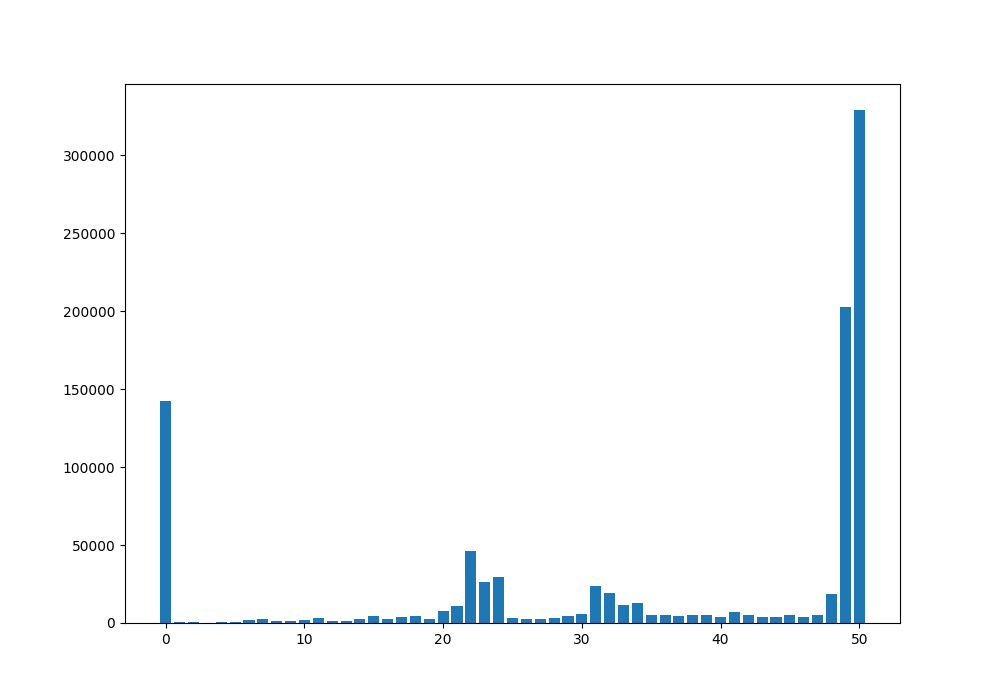
\includegraphics[width=12cm]{images/length-distr-10.png}
       \caption{Length distribution of the sequences after removing the adapter sequence with a 10\% of errors}
       \label{fig:10} 
    \end{subfigure}
    
    \begin{subfigure}[b]{1\textwidth}
       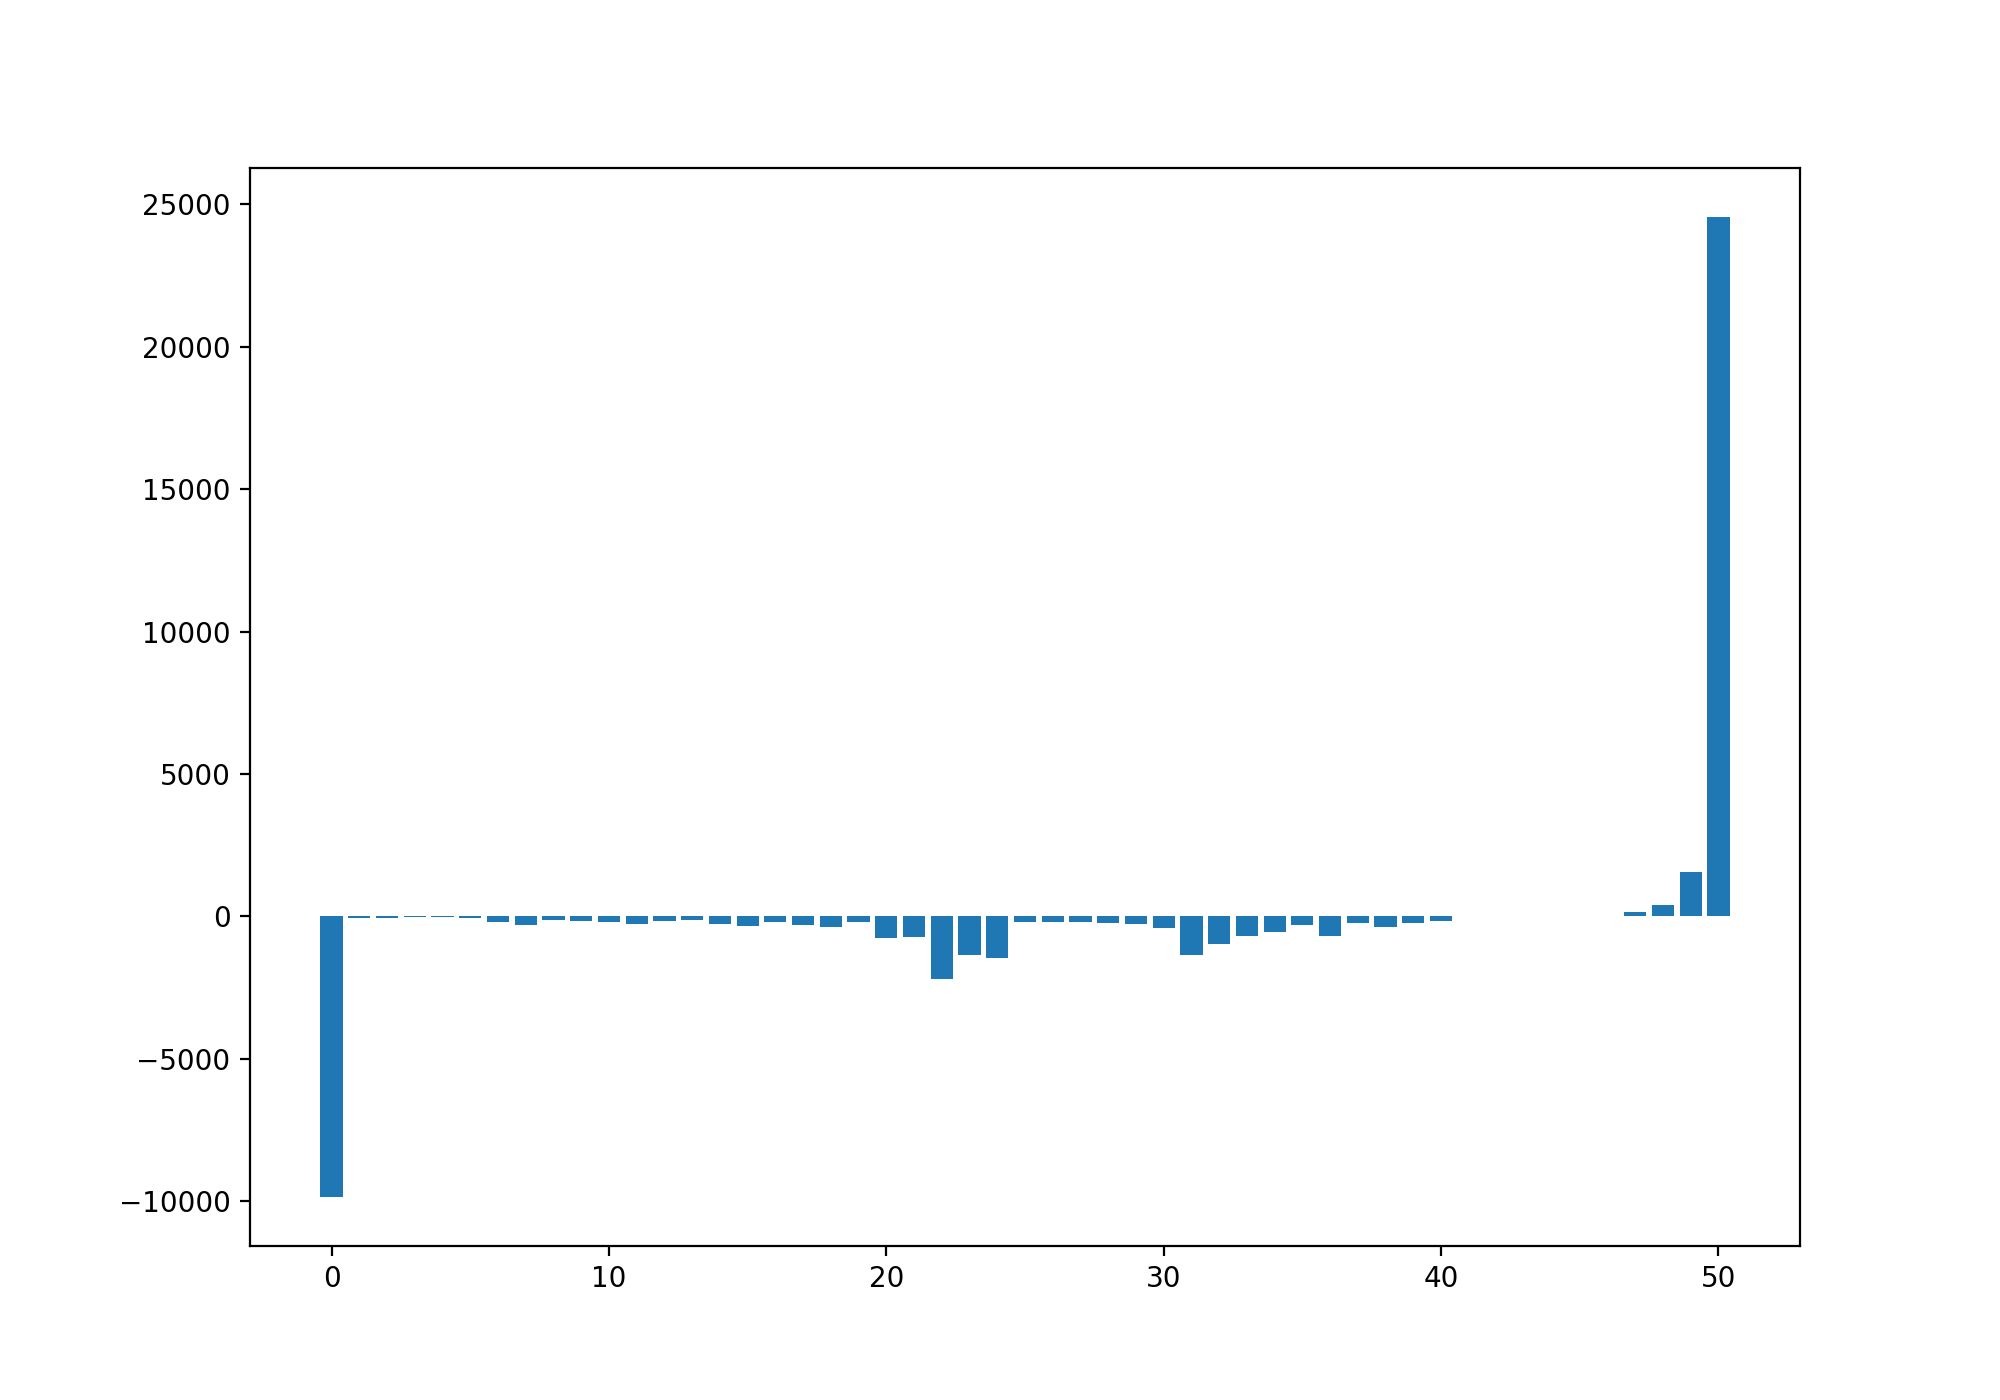
\includegraphics[width=12cm]{images/length-distr-length-distr-10.png}
       \caption{Difference between length distribution without errors and length distribution with a 10\% of errors}
       \label{fig:diff10}
    \end{subfigure}
    
    \caption{Plots for 10\% error}
\end{figure}

\begin{figure}
    \centering
    \begin{subfigure}[b]{1\textwidth}
       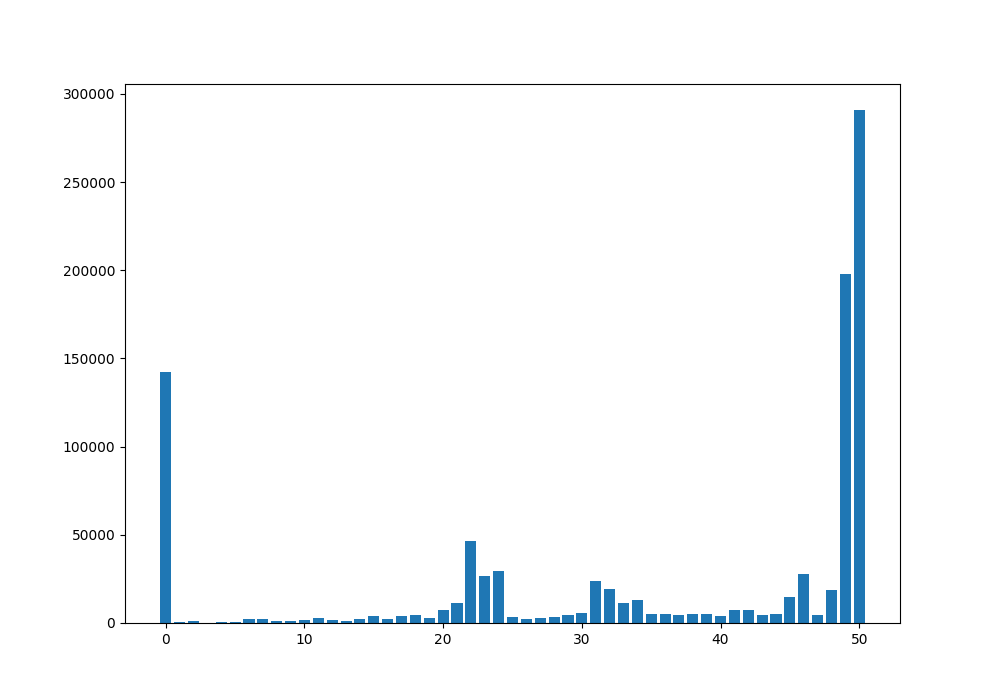
\includegraphics[width=12cm]{images/length-distr-25.png}
       \caption{Length distribution of the sequences after removing the adapter fragments with a 25\% of errors}
       \label{fig:25} 
    \end{subfigure}
    
    \begin{subfigure}[b]{1\textwidth}
       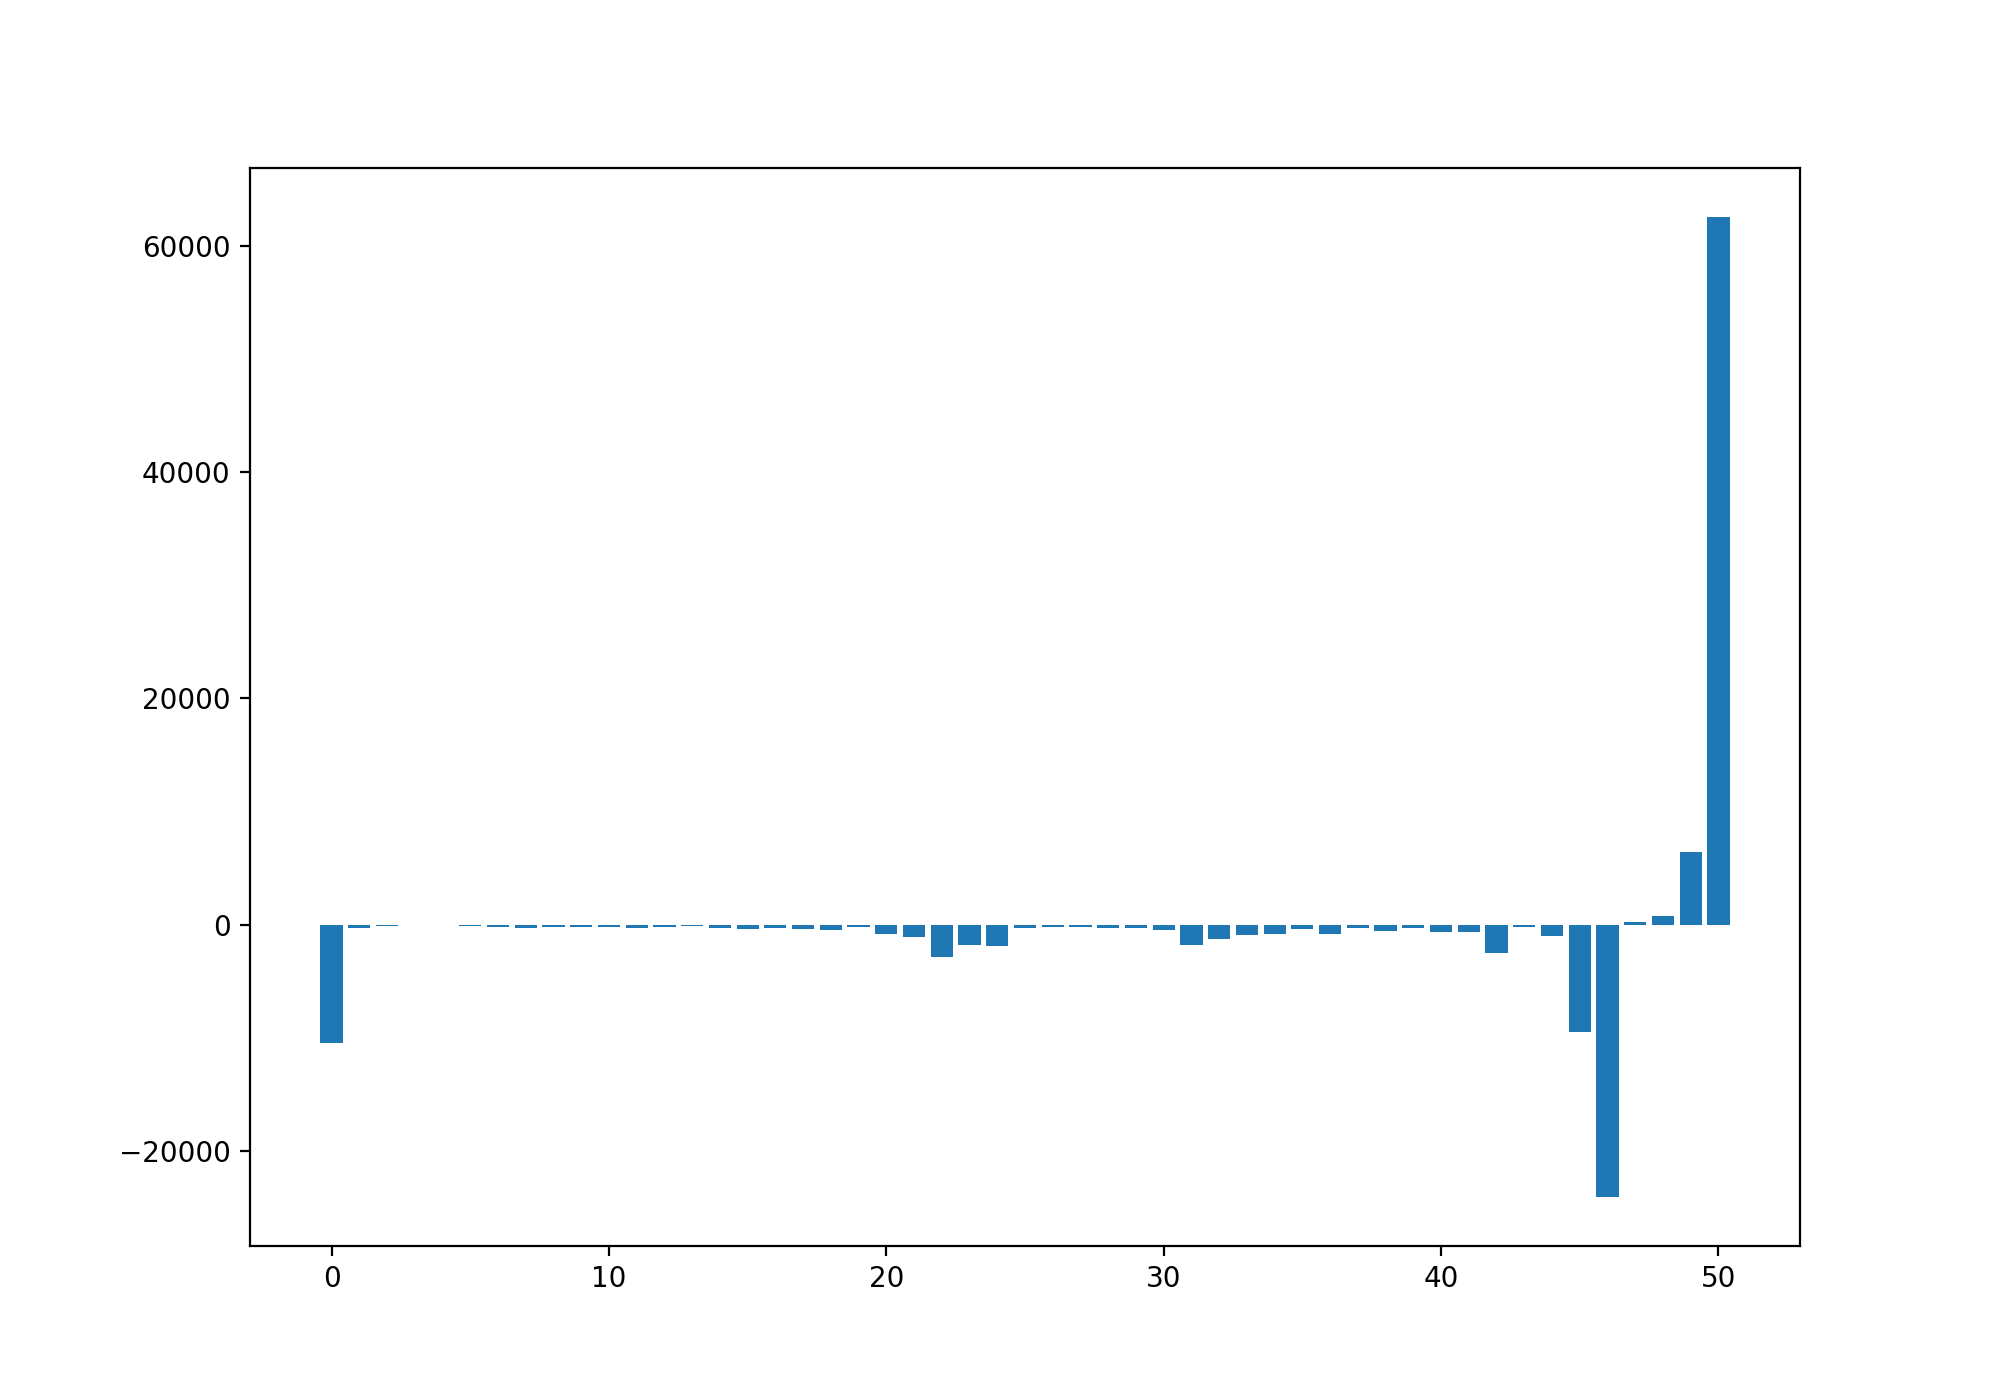
\includegraphics[width=12cm]{images/length-distr-length-distr-25.png}
       \caption{Difference between length distribution without errors and length distribution with a 25\% of errors}
       \label{fig:diff25}
    \end{subfigure}
    
    \caption{Plots for 25\% error}
\end{figure}

\begin{figure}
    \centering
    \begin{subfigure}[b]{1\textwidth}
       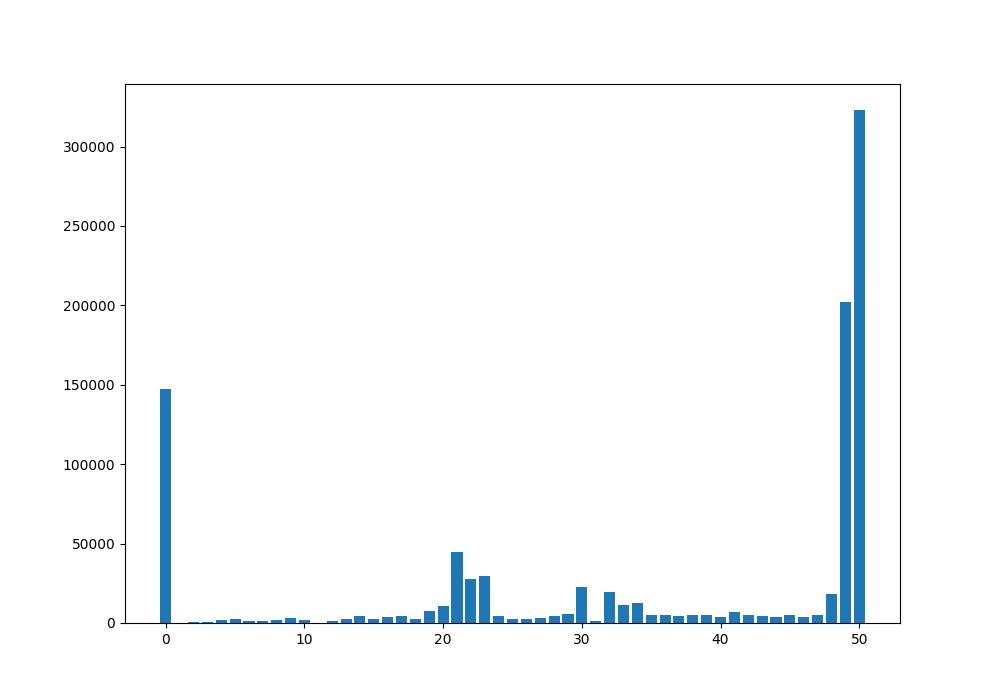
\includegraphics[width=12cm]{images/length-distr-10-id.png}
       \caption{Length distribution of the sequences after removing the adapter fragments with a 10\% of errors allowing insertions and deletions}
       \label{fig:10id} 
    \end{subfigure}
    
    \begin{subfigure}[b]{1\textwidth}
       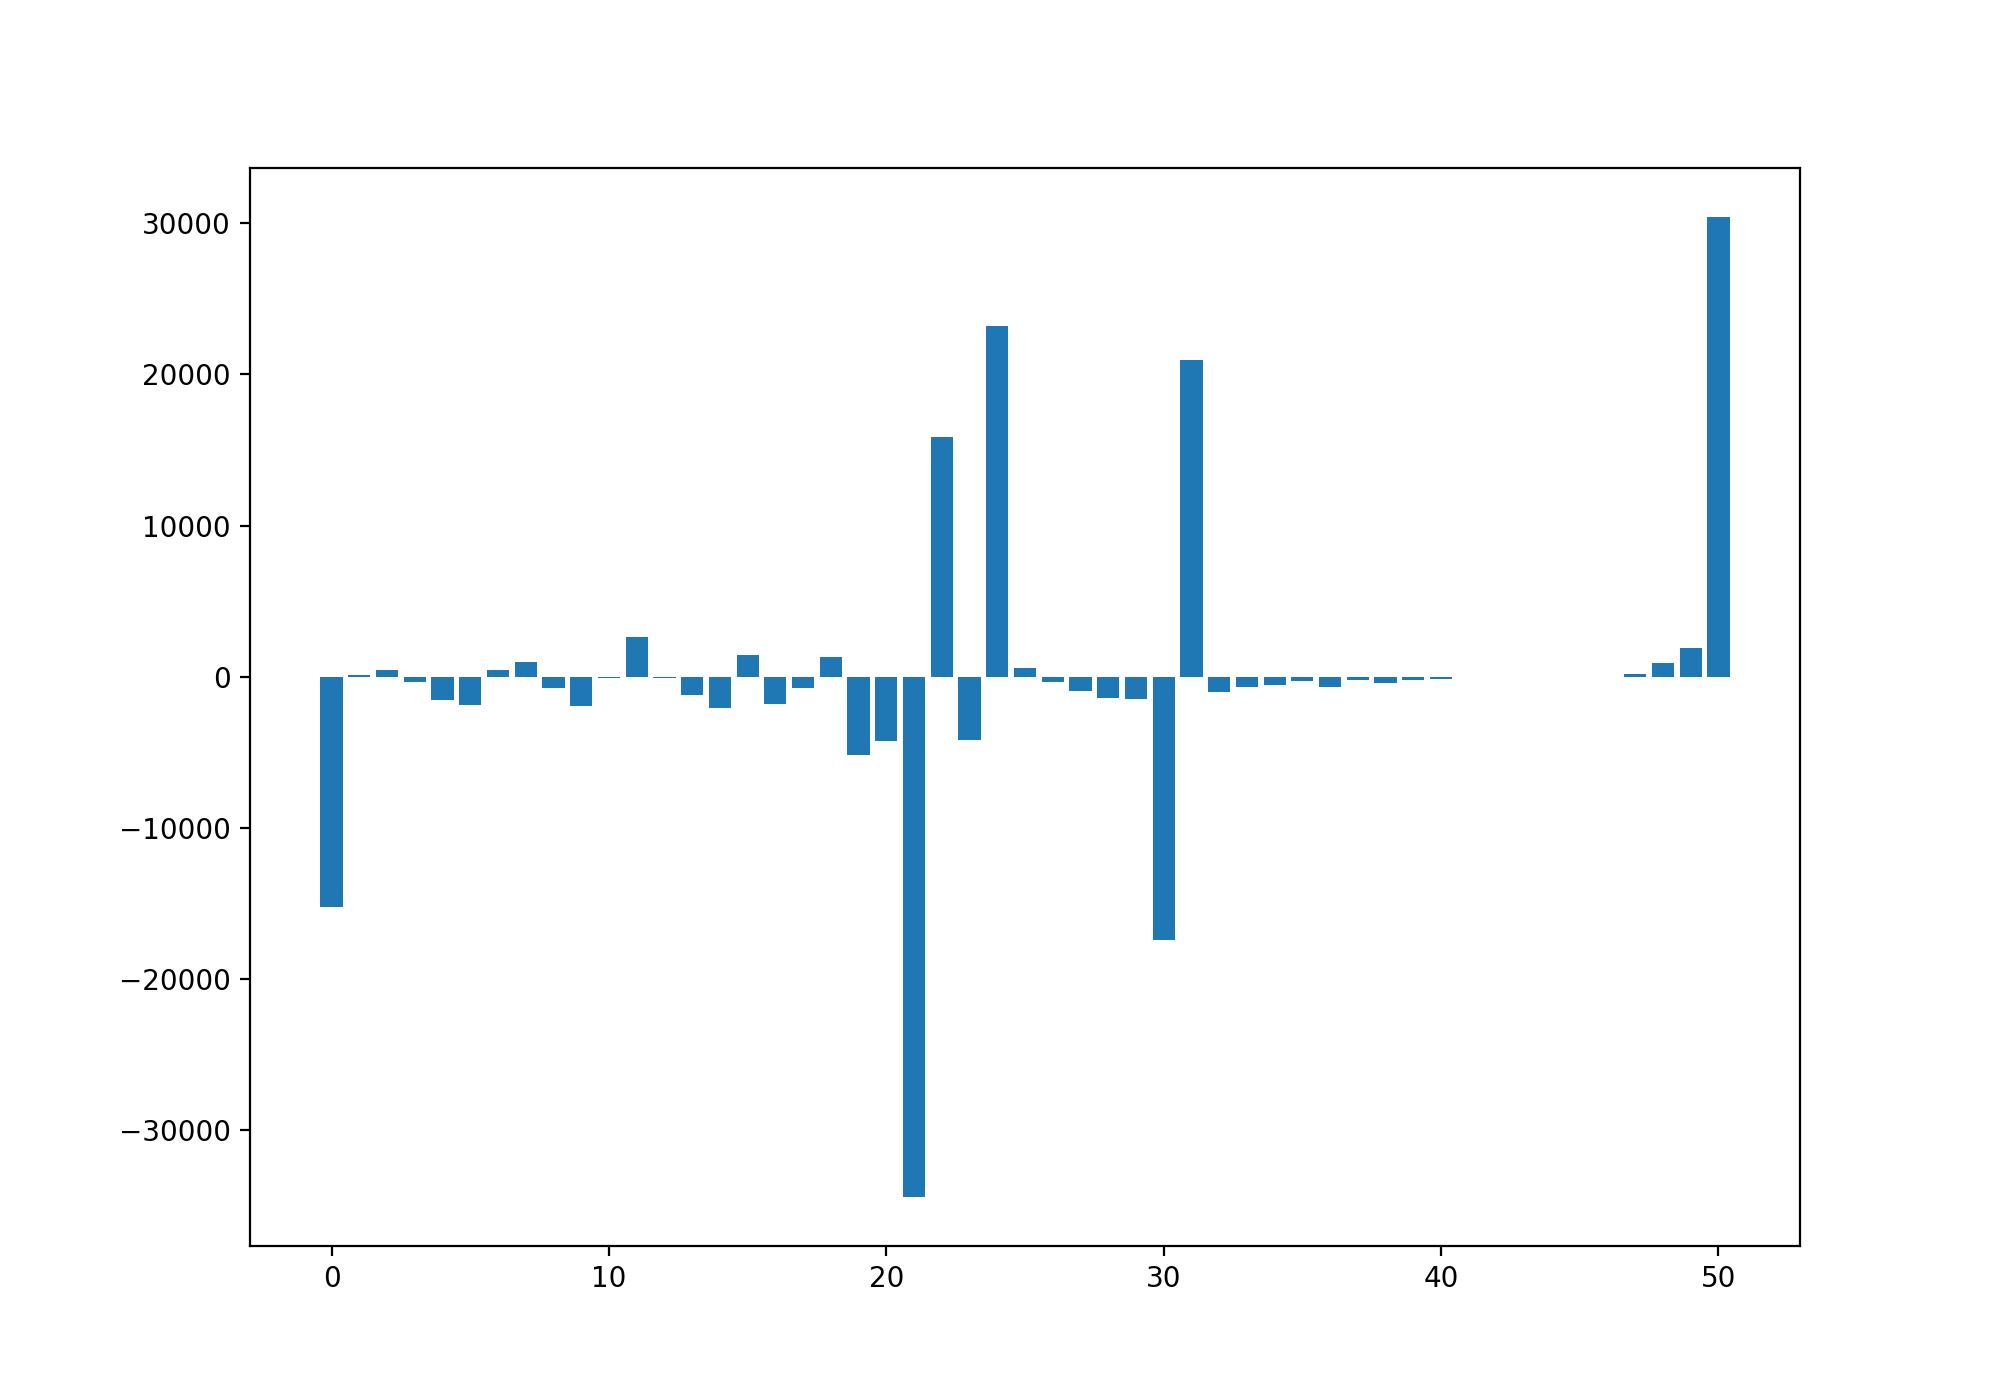
\includegraphics[width=12cm]{images/length-distr-length-distr-10-id.png}
       \caption{Difference between length distribution without errors and length distribution with a 10\% of errors allowing insertions and deletions}
       \label{fig:diff10id}
    \end{subfigure}
    
    \caption{Plots for 10\% error allowing insertions and deletions}
\end{figure}

\begin{figure}
    \centering
    \begin{subfigure}[b]{1\textwidth}
       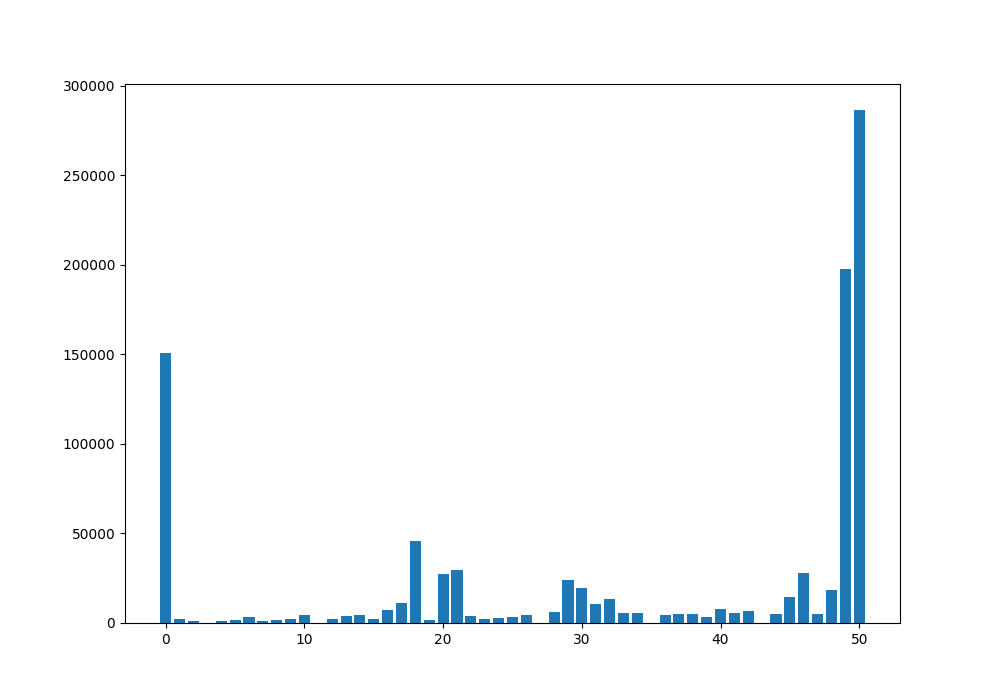
\includegraphics[width=12cm]{images/length-distr-25-id.png}
       \caption{Length distribution of the sequences after removing the adapter fragments with a 25\% of errors allowing insertions and deletions}
       \label{fig:25id} 
    \end{subfigure}
    
    \begin{subfigure}[b]{1\textwidth}
       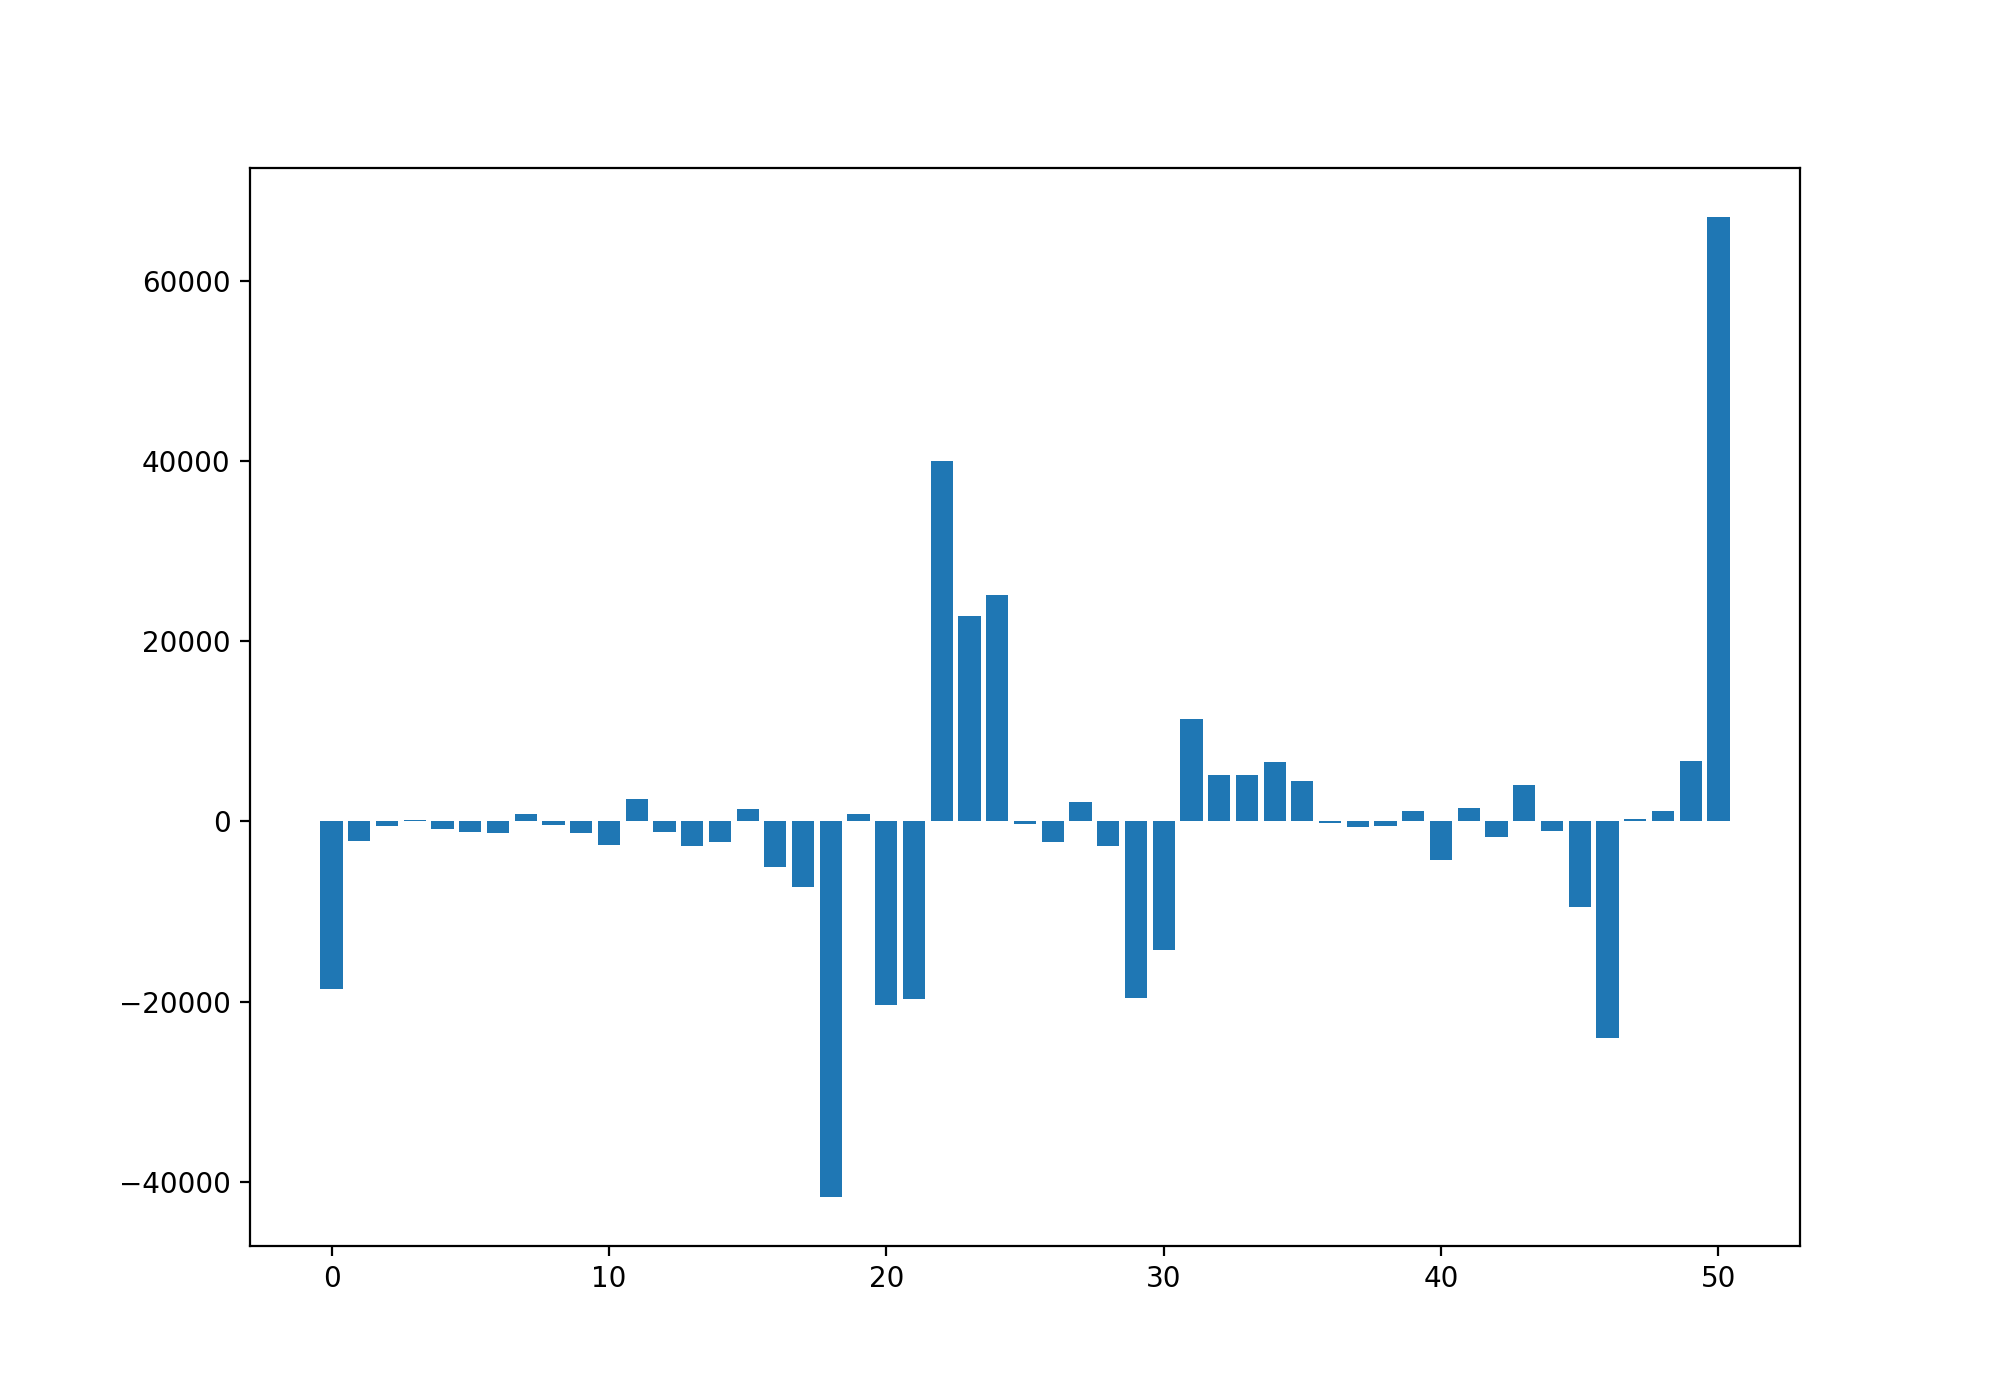
\includegraphics[width=12cm]{images/length-distr-length-distr-25-id.png}
       \caption{Difference between length distribution without errors and length distribution with a 25\% of errors allowing insertions and deletions}
       \label{fig:diff25id}
    \end{subfigure}
    
    \caption{Plots for 25\% error allowing insertions and deletions}
\end{figure}

\begin{table}[H]
    \centering
    \begin{tabular}{| c | c | c |}
        \hline
        Error & Matches & 100\% match \\
        \hline
        \hline
        0\% & 646368 & 132149 \\
        10\% & 670925 & 141997 \\
        25\% & 708900 & 142569 \\
        10\% ID & 676781 & 147408 \\
        25\% ID & 713464 & 150729 \\
        \hline
    \end{tabular}
    \caption{Matches obtained allowing errors}
    \label{table:results2}
\end{table}

\paragraph{} These are the results we have obtained with our implementation, as expected when the error percentage increases, the number of matches also increases. We can also see that the number of matches does not increase that much when we allow insertions and deletions, but if we look at the plots is precise that the distribution of the matches changes when insertions and deletions are allowed.

\newpage

\section{Task 3}

\paragraph{} The third task consists of estimating the rate estimate the rate of sequencing errors per sequence and per nucleotide and then, based on these analyses, see in which part of the sequence these errors are.

\paragraph{} We modified the code from task 2 using insertions and deletions to get the total amount of errors. The results are the following:

\begin{table}[H]
    \centering
    \begin{tabular}{| c | c | c | c |}
        \hline
        Error percentage & Total errors & Errors per sequence & Errors per nucleotide \\
        \hline
        \hline
        10\% & 462201 & 0.462 & 0.0092 \\
        25\% & 1786184 & 1.786 & 0.03572 \\
        \hline
    \end{tabular}
    \caption{Errors obtained}
    \label{table:results2}
\end{table}

\paragraph{} Seeing the results, it seems that the total amount of errors increases faster than the percentage. This could be due to the fact that the matches after the 10\% error require more amount of errors than the previous ones, this would make sense since as seen in the results of task 2 [\ref{table:results2}] when the percentage is increased the number of matches does not increase as fast.

\paragraph{} Based on the difference plots of the previous task [\ref{fig:diff10id}][\ref{fig:diff25id}] we can see that the main negative differences, meaning that with errors we get more amount of values, in the length distribution are in the center, that could mean that the errors are more likely to be there.

\newpage

\section{Task 4}

\paragraph{} In task 4, we are asked to develop an algorithm that, given a sequence set \textit{S}, identifies the most likely adapter sequence \textit{a} and use this algorithm to analyze the set found in the file tdt4287-unknown-adapter.txt.

\subsection{Most likely adapter sequence}

\paragraph{} For task 4, we created an algorithm to detect the most likely adapter sequence in a sequence set \textit{S}. This algorithm works using a simple method, if we imagine that all of the characters from a sequence are random except for the adapter sequence, we can count the number of occurrences for each character in each position in each sequence, and then the character that has the largest number of occurrences should be one from this hypothetical adapter sequence.

\begin{lstlisting}[language=c++, caption=Algortihm that finds most used character in each position from a set $S$ of strings]
void updateCount(string sequence) {
    char chars[sequence.length() + 1];

    for (uint i = 0; i < sequence.length() + 1; i++) {
        if (counts.size() < i + 1) 
            counts.push_back(vector<int>(alphabet.size()));
        char c = chars[(sequence.length()) - i];

        counts[i][idMap[c]] += 1;
    }
}

char getCharWithMoreOcc(int index) {
    int highestCount = 0, highestIndex = 0;
    vector<int> thisIndex = counts[index];

    for (uint i = 0; i < thisIndex.size(); i++) {
        int count = thisIndex[i];
        if (highestCount < count) {
            highestCount = count;
            highestIndex = i;
        }
    }
    return charMap[highestIndex];
}

string getMostCommon() {
    vector<char> res(counts.size());

    for (uint i = 0; i < res.size(); i++)
        res[i] = getMostLikely(i);
    
    string finalAdapterSequence = "";
    for (int i = res.size() - 1; i >= 0; i--)
        finalAdapterSequence.put(res[i]);

    return finalAdapterSequence;
}
\end{lstlisting}

\paragraph{} The code works as we first process the sequence (and we do this for each sequence of the set $S$), in this process function we take each sequence and we map them with the number of occurrences per each character in that position in specific, then for each index of the sequence we search from the alphabet ${[A, C, G, T, N]}$ the character with the most number of occurrences, and finally, at each position of the result vector, we put the result of the most likely character for that position in specific having the final estimated adapter sequence.

\subsection{Results}

\paragraph{} To know if our algorithm works, we tested it by trying to find the adapter sequence in s-3-sequence-1M.txt, so we used the data sets used in $Task 1-2$ trying to find the estimated adapter sequence for this data set. The results for this last task are shown in Listing \ref{lst8:label}. We can see that the result is very similar to the original adapter.

\begin{lstlisting}[language=c++, caption=Results for the most likely adapter sequence algorithm in 's-3-sequence-1M.txt' , label={lst8:label}]
1: Testing algorithm for a sequence with a known adapter
Sequence found: TGGAATTGTTGAATGCCAAGGGCTTCCAGTCACAGAGTGTTCTAATATGCA
\end{lstlisting}

\paragraph{} Applying this to the 'tdt4287-unknown-adapter.txt' we get the result shown in Listing \ref{lst9:label}. And when applying it to 'seqset3.txt' we get the result in Listing \ref{lst10:label}.

\begin{lstlisting}[language=c++, caption=Results for the most likely adapter sequence algorithm in 'tdt4287-unknown-adapter.txt', label={lst9:label}]
3: Finding the most likely adapter in 'tdt4287-unknown-adapter.txt'
Most likely adapter sequence: TAAAGGATAAGCAGCCGACGTGGGGCGGGTCGAAAAGCGTTAGGATTACTGAGTAGATCGGAA-GAGCACACGTCTGAACTCCAGTCACGTAGAGATCTCGTATGCCGTCTTCTGCTTGAAA 
\end{lstlisting}

\begin{lstlisting}[language=c++, caption=Results for the most likely adapter sequence algorithm in 'seqset3.txt', label={lst10:label}]
4: Finding sequence in 'seqset3.txt'
Sequence found: CCCGGGGCGGGAAAGTTTGGGTTGGAAATCTCGGGGGCCAAAAAACCCCCCA 
\end{lstlisting}

\paragraph{} When exploring the most common suffixes we can find 3 different common suffixes when executing it in the data set 's-3-sequence-1M.txt' shown in Listing \ref{lst11:label}.

\begin{lstlisting} [language=c++, caption=Results for most common suffixes, label={lst11:label}]
5: Most common suffixes:
Sequence found: TGGAATTGTTGAATGCCAAGGGCTTCCAGTCACAGAGTGTTCTAATATGCA
Sequence found: CTTGGAGAAGAGCAAAATTTTAACGAGTACACTGATTAAGGGGGTATCCTT
Sequence found: GCCCTGACGCTTGCTTGGCAATTGCGAGTATGGTTCCCCCCTCTCGCAAAC
\end{lstlisting}


\paragraph{} If we remove all the adapter sequences from our pre-set sequences we get the length distribution in Figure \ref{fig:ld4}.

\begin{figure}[H]
    \centering
    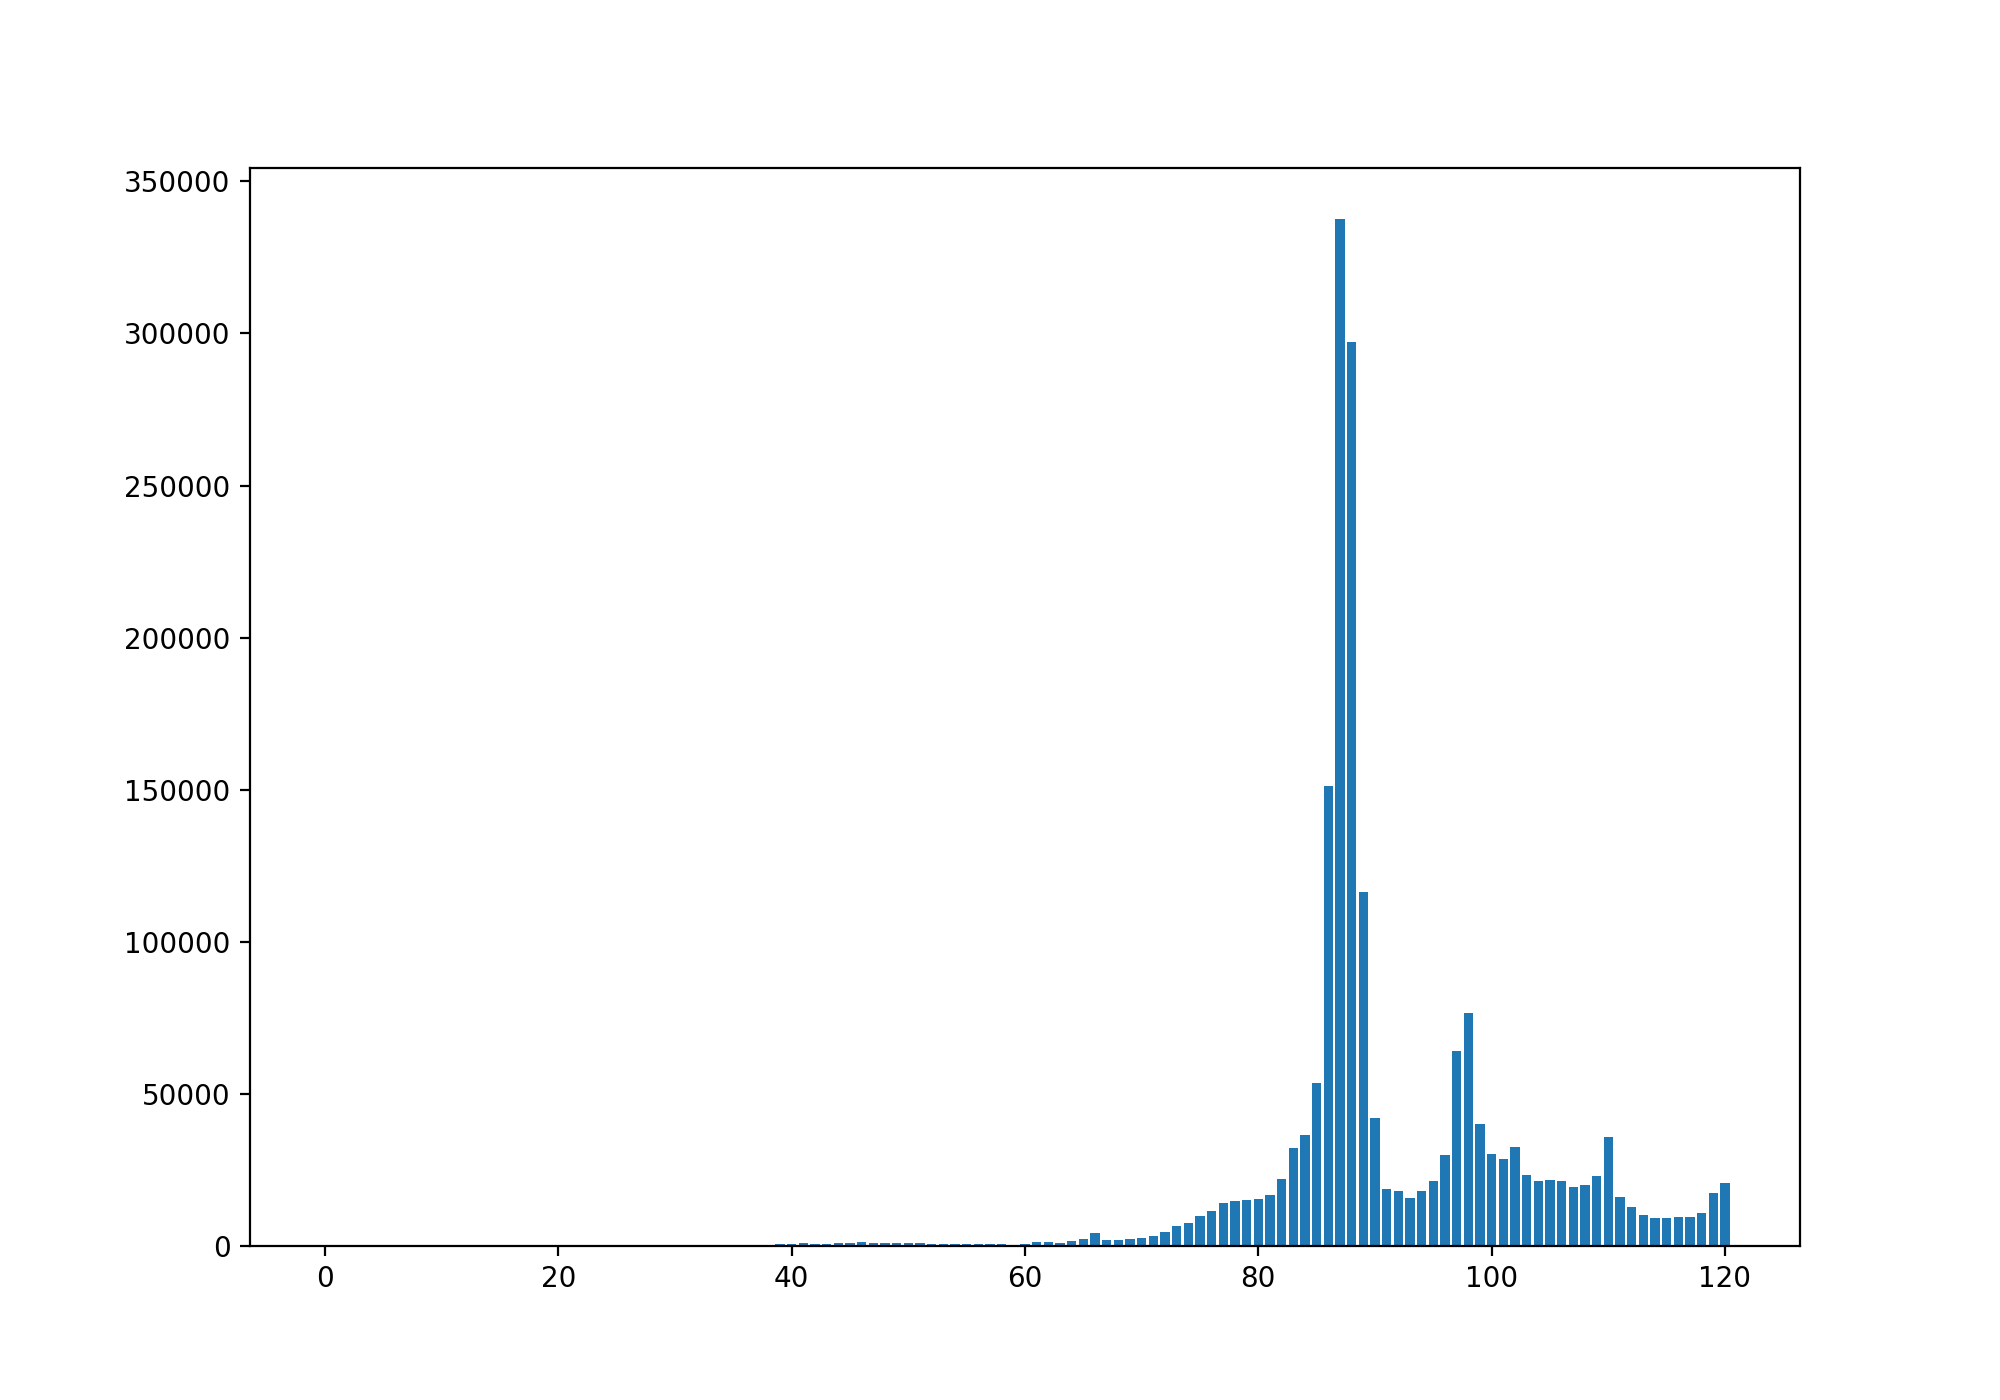
\includegraphics[width=12cm]{images/length-distr-task4.png}
    \caption{Length distribution of the sequences after removing the adapter fragments}
    \label{fig:ld4}
\end{figure}

\paragraph{} For the frequency distribution for the data set of 'tdt4287unknown-adapter-sequence.txt' we can see the results in Figure \ref{fd}.

\begin{figure}[H]
    \centering
    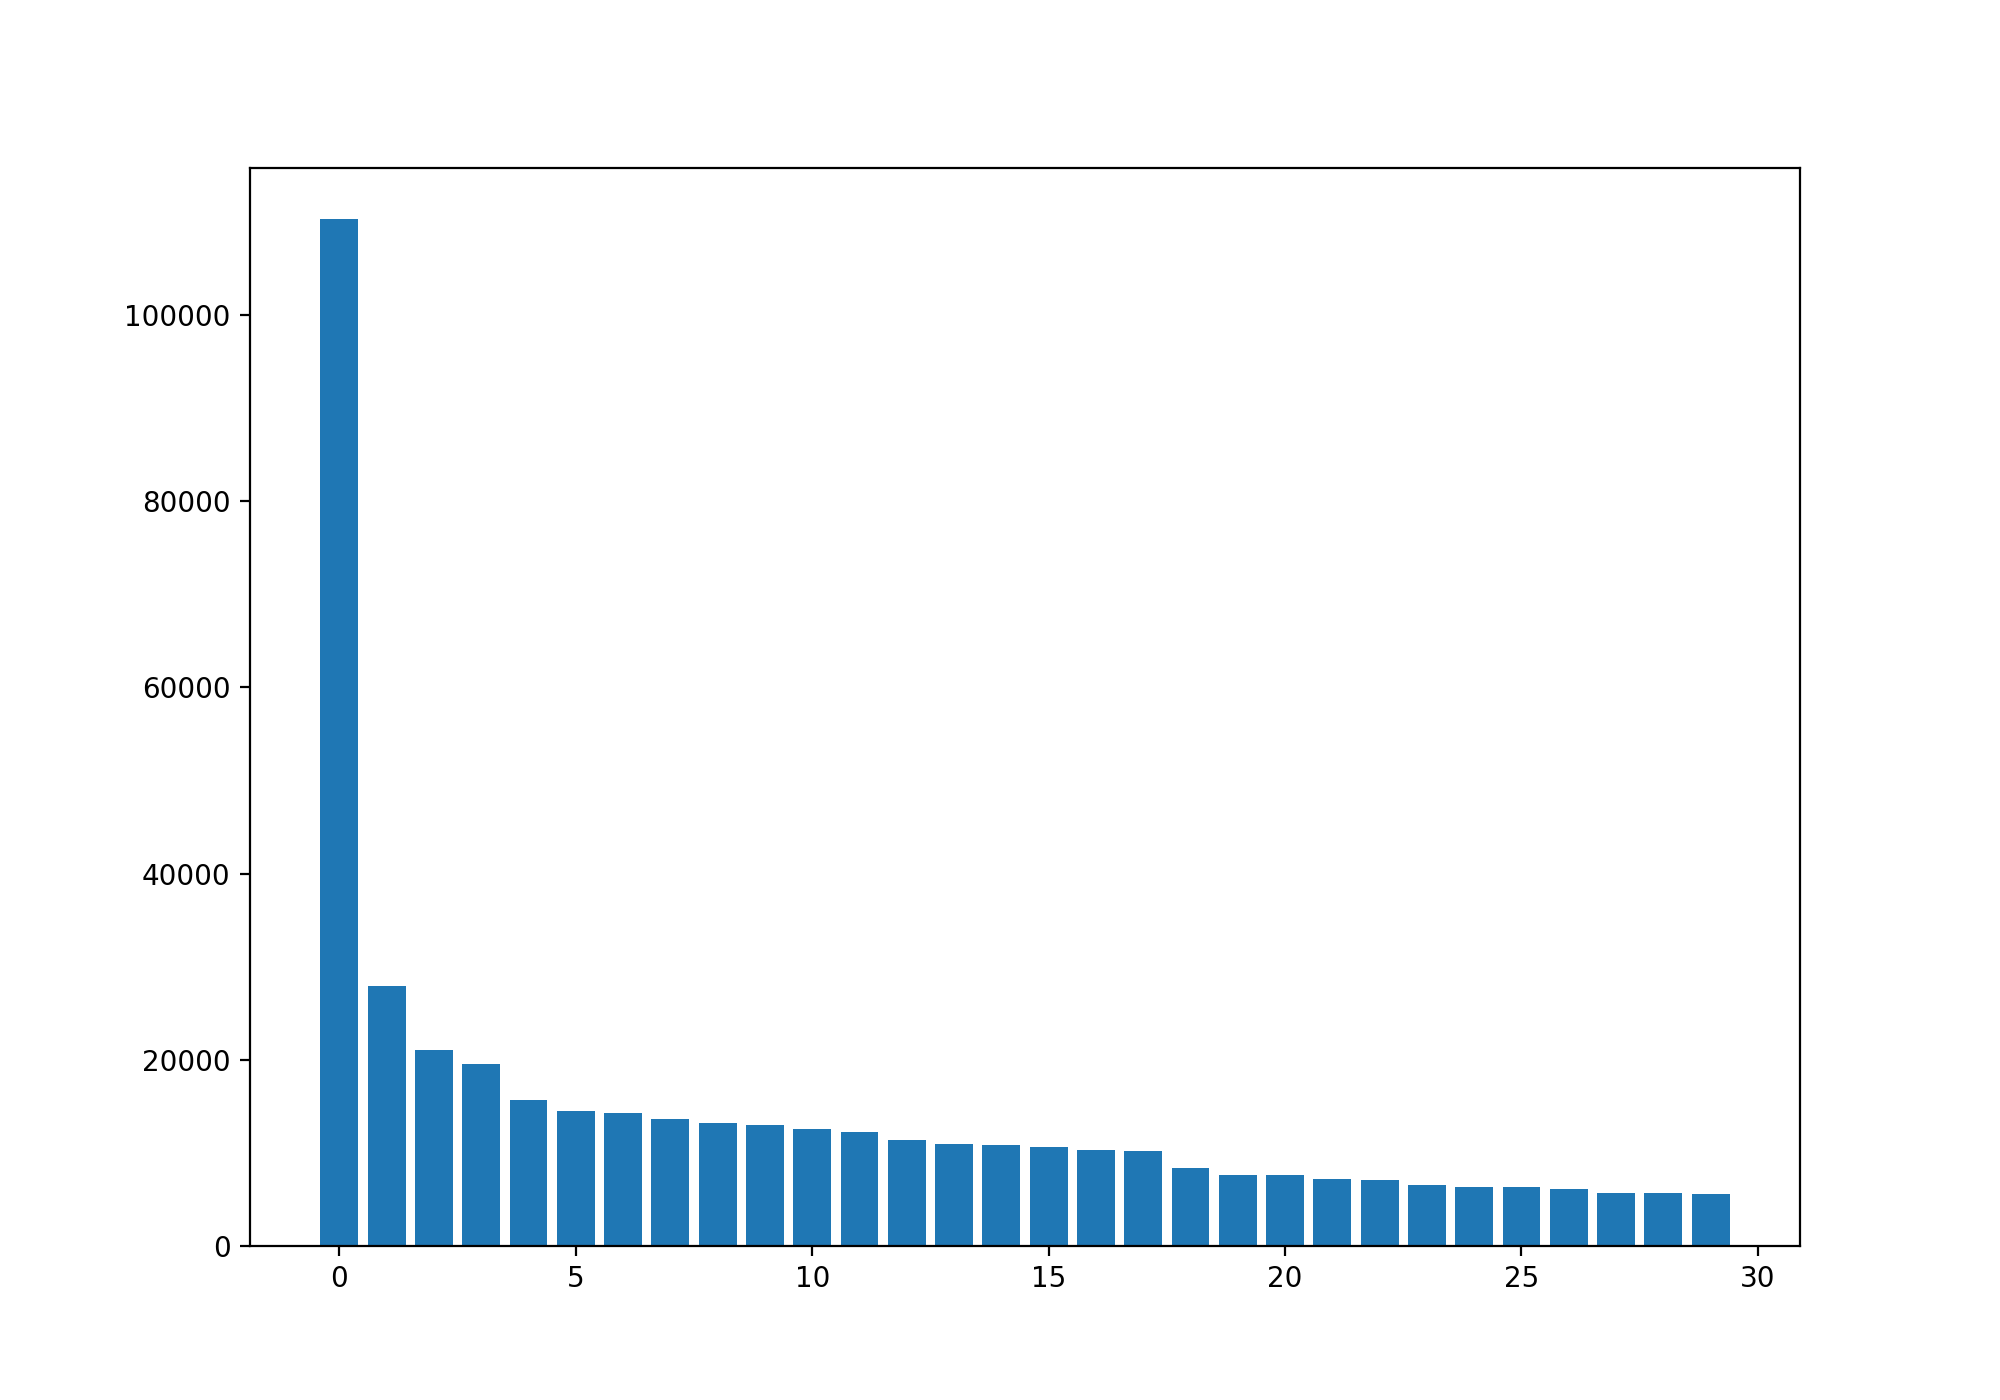
\includegraphics[width=12cm]{images/freq-distr.png}
    \caption{Frequency distribution of the 'tdt4287unknown-adapter-sequence.txt' data set}
    \label{fig:fd}
\end{figure}

\paragraph{} Finally we expose the algorithmic cost of our procedure where the worst asymptotic running time for it is $O(nk)$ where $n$ is the number of sequences that we have to process and $k$ is the length of the sequences.

\newpage

\section{Task 5}

\paragraph{} In Task5 we were asked to identify the barcodes and how many samples were multiplexed, to identify how many sequences were sequenced from each sample, and to identify the sequence length distribution within each sample. All of this information is to be extracted from the 'MultiplexedSamples.gz' data set.

\subsection{De-Multiplexed barcode library}

\paragraph{} For this task we have developed an algorithm that identifies all barcodes from a data set $S$. This algorithm works using a different approach from the algorithm on Task4, as it uses an $multiLCS$ to determine the sequences that are going to be examined to search for those barcodes. We can see a pseudo-code in Listing \ref{lst12:label}.

\begin{lstlisting}[language=c++, caption=Algorithm to identify the barcodes and the sequences multiplexed, label={lst12:label}]

pair<vector<string>, vector<string>> identifyBarcodes(vector<string> sequences) {
    vector<string> barcodes;
    vector<string> copyOfSequences;
    for (uint i = 0; i < sequences.size(); i++) {
        copyOfSequences.push_back(sequences[i]);
    }

    while (true) {
        if (copyOfSequences.empty()) {
            for (string seq : sequences) {
                barcodes.push_back(seq.substr(-BARCODE_LENGTH, 
                                                seq.length()));
                seq = seq.substr(0, seq.length() - BARCODE_LENGTH);
            }
            break;
        }
        string lcs = multi_lcs(copyOfSequences);

        if (lcs.empty())
            break;

        vector<int> indexes;
        for (uint i = 0; i < copyOfSequences.size(); i++) {
            uint startIndex = copyOfSequences[i].find(lcs);
            if (startIndex != string npos) {
                sequences[i] = copyOfSequences[i].substr(0, startIndex + 1);
                indexes.push_back(i);
            }
        }
        uint sizeOfCopy = copyOfSequences.size();
        copyOfSequences.clear();
        for (uint i = 0; i < sizeOfCopy; i++) {
            if (find(indexes.begin(), indexes.end(), i) != indexes.end())
                copyOfSequences.push_back(sequences[i]);
        }
    }
    return make_pair(barcodes, sequences);
}

\end{lstlisting}

\paragraph{} This code identifies the barcodes and the sequences that are multiplexed for the data-set $S$, as it takes from arguments a vector with the lines of the file read before.
In this code, we use an auxiliary vector $(copyOfSequences)$ to make different operations without corrupting the important one. As we said earlier, we use a $multiLCS$ (Listing \ref{lst13:label}) to determine which sequences will treat. We use an index vector to keep track of the sequences marked with the $LCS$. Then in sequences, we add this substring created from 0 to where we found our $LCS$ value, and finally, we save that sequence index to our vector of indexes. When we are finished with creating all substrings and getting the correct indexes, we clear the vector of $copyOfSequences$ and push back only the sequences in $sequences$ that have an index inside $indexes$, and we will do this until all sequences are treated. We will finish treating all these sequences at one point, and no more sequences will be stored in $copyOfSequences$. Then at this point, we will loop for each sequence in $sequences$ and add to the $barcodes$ vector the substring from the last 4 $<=$ BARCODE-LENGTH $<=$ 8 characters and updating that sequence removing that substring from it.\\
Finally, after doing all that process, we will have a vector with all the identified barcodes and a vector with all the sequences without all these barcodes, all the sFigure 8: Length distribution of the sequences after removing the barcodesequences multiplexed.

\vspace{5mm} %5mm vertical space

\paragraph{} Referring to the algorithmic cost of the procedure, we have to take into account that we are using a $LCS$ that has a time complexity of $O(nm)$ being $n$ and $m$ the sizes of both strings to compare or the sizes for each of the compare operations that have to be done for example in a big data-set case. Knowing that our algorithm also consumes a $O(nk)$ being $n$ the number of sequences to be processed and $k$ the size of each sequence. So we have an algorithmic cost of $O(nk + nm) = O(nk)$.

\begin{lstlisting}[language=c++, caption=Multi LCS algorithm, label={lst13:label}]
string multi_lcs(vector<string> sequences) {
    // Size of the array
    uint n = sequences.size();

    string s = sequences[0];
    uint l = s.length();
    string res = "";

    for (uint i = 0; i < l; i++) {
        for (uint j = i + 1; j < l + 1; j++) {
            // Generating all possible substrings of our reference string s
            string aux = s.substr(i, j-i);
            uint k;
            for (k = 1; k < n; k++) {
                // Checking if the generated aux is common to all words
                if (sequences[k].find(aux) == string npos)
					break;
            } 
			// If the current substring is present in all strings and its length
            // is greater than the current result
            if (k == n && res.length() < aux.length())
                res = aux;
        }
    }
    return res;
}
\end{lstlisting}

\subsection{Results}

\paragraph{} After the execution of our code, we got different results depending on the length of the barcode that can be, as explained before in an interval of $4 <= BARCODELENGTH <= 8$, and also the number of sequences represented per barcode, because as we can see in Listing \ref{lst14:label} each barcode has a pair associated that represents the number of sequences that match once these barcodes were removed.\\
\\
It has to be taken into account that we are working without unique sequences so some barcodes such as AAAA have an enormous amount of appearances in sequences such there are duplicated sequences in the input data set.

\vspace{5mm} %5mm vertical space

\begin{lstlisting}[language=c++, caption=Results for the barcode identifying process, label={lst14:label}]
Barcodes and sequences represented per barcode:

8: [[AAACCCCT, 7], [GGCATTTC, 0], [TCGGGGGG, 0], [CTTTAAAA, 12886]]

7: [[AACCCCT, 3], [GCATTTC, 4], [CGGGGGG, 0], [TTTAAAA, 149]]

6: [[ACCCCT, 0], [CATTTC, 2], [GGGGGG, 0], [TTAAAA, 347]]

5: [[CCCCT, 1], [ATTTC, 0], [GGGGG, 0], [TAAAA, 10220]]

4: [[CCCT, 2], [TTTC, 3], [GGGG, 4], [AAAA, 6048973]]
\end{lstlisting}

\paragraph{} For the length distribution within each sample can be measured depending on the length of the barcode that has been removed because as we know for the data set 'MultiplexedSamples.gz' all sequences share the same length so if we remove two barcodes that also share lengths the length distribution will be the same. So in the next Figure \ref{fig:t5res} we have the distribution for each length(4 to 8).

\begin{figure}[H]
    \centering
    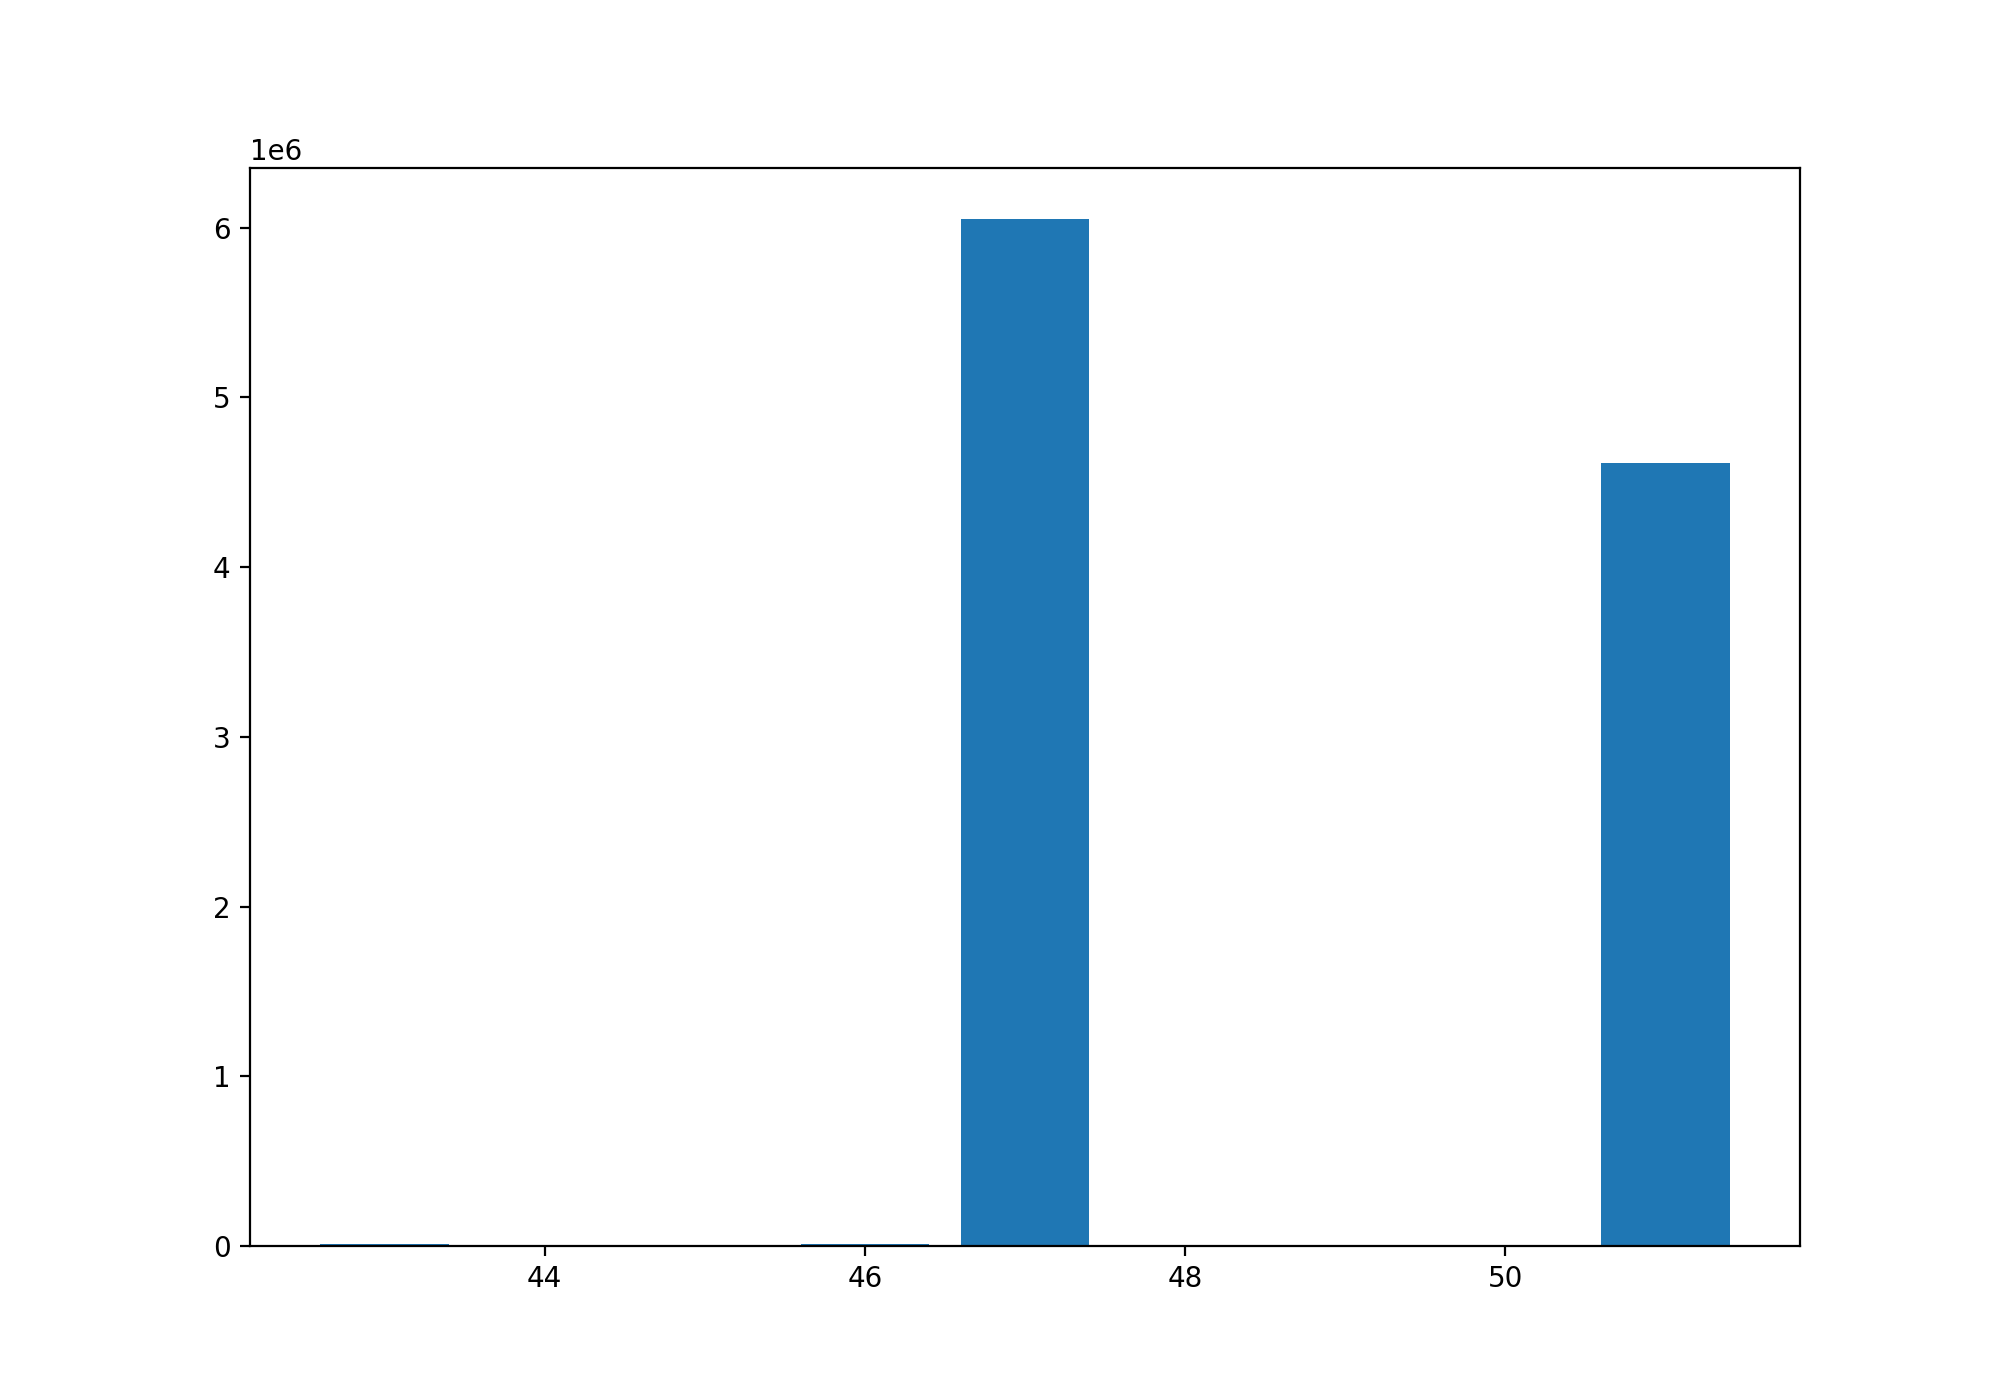
\includegraphics[width=12cm]{images/length-distr-task5.png}
    \caption{Length distribution of the sequences after removing the barcodes}
    \label{fig:ld4}
\end{figure}

\newpage

\listoffigures

\listoftables

\end{document}
